\documentclass[10pt]{article}\usepackage[margin=.65in]{geometry}\usepackage[T1]{fontenc}\usepackage{graphicx}\setlength{\parindent}{0pt}\setlength{\parskip}{7pt}\sloppy\begin{document}{\large State preservation, repair closure and Cantor reduction}\par This packet composes three source-linked mathematical components and one saved-data accounting audit. It retains the full 1,260-target scope. No scientific cohort, solver trajectory, or cloud workload was executed. The prospective review plan was published at 6f7a9eec4f; the accounting review joint was added with its source publication.\par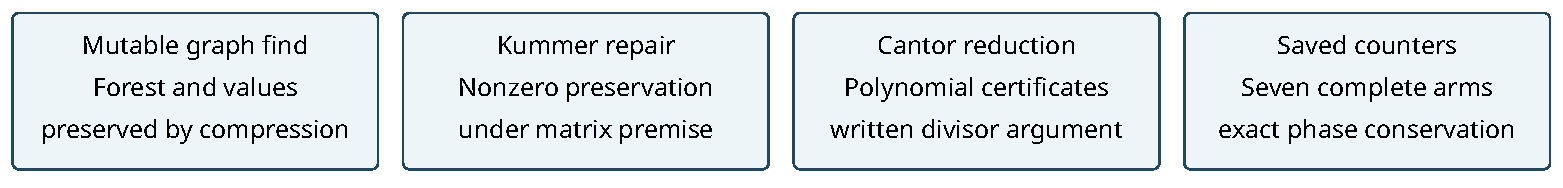
\includegraphics[width=\linewidth]{diagram.pdf}\par Mutable graph find: two main theorems and eight controls establish whole-state preservation of the rank-decreasing forest and node-value equations. The execution relation follows native read-parent, recurse, post-recursion child-potential read, and both writes. A frame property justifies that recursive compression does not change the child before its read. A separate theorem establishes finite successful execution.

Kummer repair: ten field theorems and nine controls prove nonzero preservation and reflection for the literal four-coordinate linear action when its matrix square is cI with c nonzero. Comparator preservation and reflection and the corrected degree-two/degree-one chart basis identity are included. Concrete runtime matrix binding and full word-fold semantics remain separate.

CZero Cantor: twelve declarations and six controls give the full two-Bezout-stage composition numerator, degree bounds, unique exact quotient, and negative remainder certificate. A separate written argument derives div(y-ell)=D1+D2+R-5O and div(X-x)=R+Rprime-2O under smooth odd-characteristic quintic assumptions, including multiplicities and infinity. The resulting divisor-class interpretation is written mathematics, not a mechanized geometric carrier.

Saved phase accounting: seven frozen arms each retain 1,260 target records. All 8,820 candidate records and their rho records conserve every recorded counter across named phases. The native reporter rejects structural duplicates and emits issues for mismatches; acceptance additionally requires exactly the seven full arms and no issues or unresolved rows. Counter conservation does not establish complete physical instrumentation or supply a new cost ratio.

Independent reviews passed 25 graph readbacks, 24 Kummer readbacks and 25 Cantor readbacks. The written geometric argument was reviewed separately. Independent native accounting replay matched all 17,640 conservation checks and rejected eight malformed inputs through an explicit acceptance gate. Each component retains exact source and input bindings, failed attempts, controls, separate readbacks, inspected PDF and editable SVG. Reviews distinguish field and scalar-state semantics, native execution, geometric interpretation and evidence-workflow completeness.

Campaign limits remain expired at 2026-10-31 06:00 UTC. Current-main integration remains a shared session-log conflict, and the prior attempted merge was aborted without modifying either history. The packet-local journal records work while the shared-log reservation remains unresolved.

A verification-wrapper defect was reproduced: the old graph helper returned shell zero after a Lean failure. A separately published replacement uses fresh invocation directories and propagates native failures; its independent review passed two genuine invocations and four boundary cases. Empty Lean inputs may compile, but the explicit source-and-ten-declaration acceptance predicate rejects them. Early setup exception receipt behavior remains outside that scoped repair. A scoped source scan records ten historical helpers with the same pattern, including a retained failed early comparator control; later successful native receipts remain separate. Old evidence is unchanged.
\end{document}